\section{Einleitung}
In den vorherigen Kapiteln wurde gekl\"art welche Anforderungen an \mops gemacht werden. In dem nun folgenden Kapitel wird eine Idee pr\"asentiert wie diese Komponenten miteinander interagieren sollen. Um einen groben \"Uberblick \"uber die Idee zu verschaffen soll dieses Kapitel mit einem Bild eingeleitet werden.
\begin{figure}[h!]
	\centering
	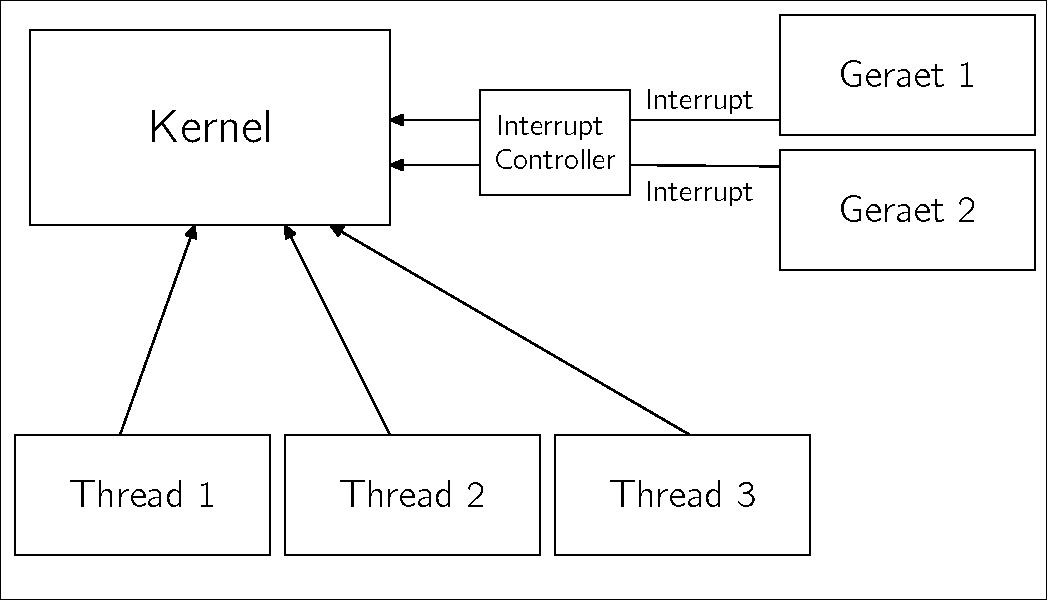
\includegraphics[scale=0.60]{common/draft-overview.pdf}	
	\caption{\mops \"Uberblick}
	\label{draft:overview}
\end{figure}\\
\mops besteht im Gro\ss en und Ganzen aus vier \"ubergeordneten Komponenten. 
\begin{dinglist}{227}
	\item{\textbf{Ger\"ate}} \\ 
	Wie in den Anforderungen beschrieben besteht \mops auf zwei Hardwarekomponenten. Diese Komponenten k\"onnen Interrupts ausl\"osen um mit dem Betriebssystem zu kommunizieren.
	\item{\textbf{Interrupt Controller}} \\
	Damit kommen wir zu einem weitern Punkt der \mops pr\"agt. Der Interrupt-Controller ist, wie in den Anforderungen beschrieben, eine Hardwarekomponente die auf den Chip integriert ist und die Priorisierung und Weiterleitung von Interrupts an das Betriebssystem steuert.
	\item{\textbf{Threads}} \\
	Die Threads stellen unter anderem die User-Programme in dem Betriebssystem dar. Sie k\"onnen mit dem Kernel interagieren und werden von dem Kernel verwaltet.
	\item{\textbf{Kernel}} \\ 
	Der Kernel ist der Hauptbestandteil von \mops, er stellt die Schnittstelle zu s\"amtlicher Hardware und den Threads dar.
\end{dinglist}
\section{Ger\"ate}
Die Ger\"ate stellen neben dem Kernel und den Threads eine sehr wichtige Rolle in \mops dar. Die Ger\"ate k\"onnen \"uber Interrupts mit dem Kernel kommunizieren. Hierbei handelt es sich um eine hardware-basierte Interprozesskommunikation.
\section{Interrupt-Controller}
Wie aus der Abbildung \ref{draft:overview} ersichtlich liegt zwischen den Ger\"aten und Kernel der sogenannte Interrupt-Controller, eine Hardwarekomponente die die Priorisierung und Verwaltung von Interrupts \"ubernimmt. In der Idee von \mops hat der Interrupt-Controller die Funktion die Quellen der Interrupts zu lokalisieren und die passenden Interrupt-Service-Routine bereitzustellen, sodass diese von dem Kernel ausgef\"uhrt werden k\"onnen. Abbildung \ref{draft:draft-vic} soll das verdeutlichen.
\begin{figure}[h!]
	\centering
	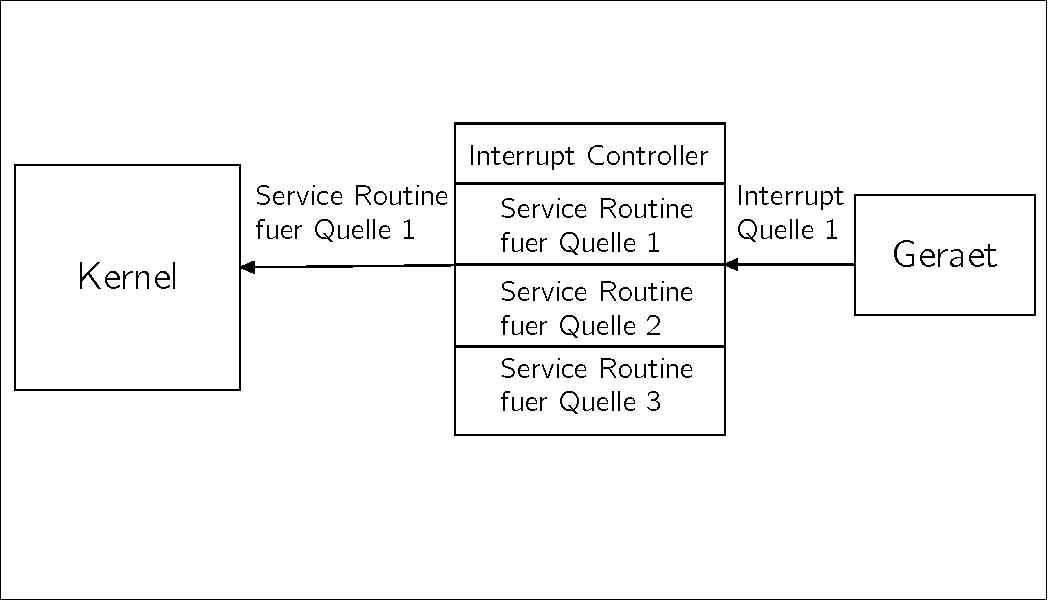
\includegraphics[scale=0.60]{common/draft-vic.pdf}	
	\caption{Interrupt-Controller}
	\label{draft:draft-vic}
\end{figure}
\newpage
\section{Threads}
In den Anforderungen wurde beschrieben das \mops aus drei Threads besteht. Diese Threads stellen User-Programme dar die \"uber bestimmte Routinen mit dem Kernel kommunizieren jedoch aber auch von Interrupts unterbrochen werden k\"onnen. Ein Thread ist in \mops, wie auch in vielen anderen Betriebssystemen, ein Abbild von einem Prozess der definierte Aktionen ausf\"uhrt, z.B. eine Berechnung oder eine Ausgabe. Damit diese Aufgabe nicht der Kernel \"ubernehmen muss existieren eben genannte Threads. Aufgrund der Tatsache das \mops keine Festplatte oder ein anderes dauerhaft beschreibbares Medium besitzt, m\"ussen die Threads alle in den RAM geladen werden. Die Idee von \mops war es also die Threads in einen definierten Bereich im RAM zu laden. Die folgende Abbildung zeigt diesen Sachverhalt.
\begin{figure}[h!]
	\centering
	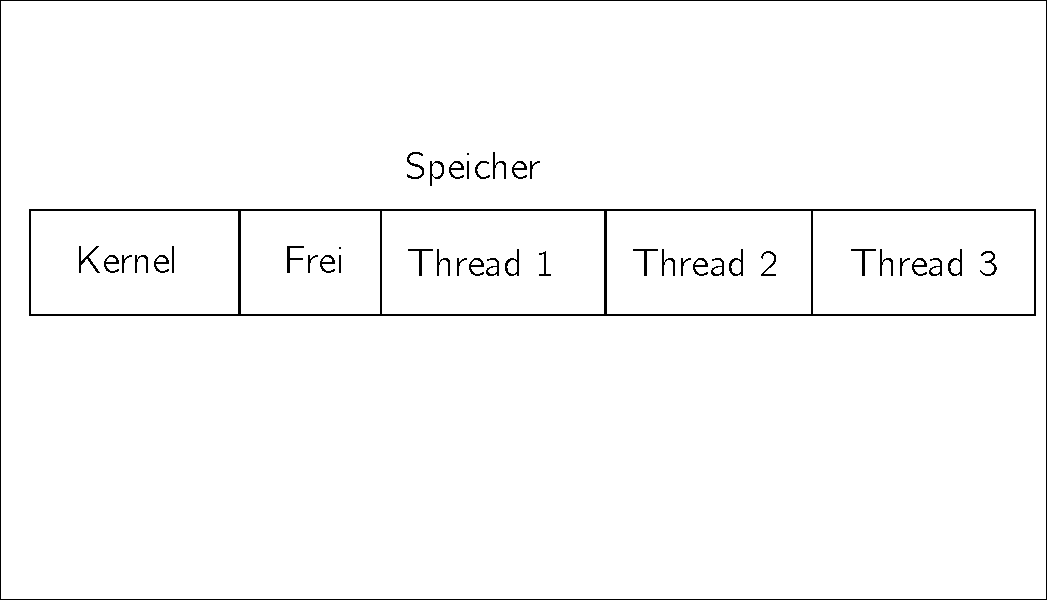
\includegraphics[scale=0.60]{common/draft-thread-overview.pdf}	
	\caption{Thread-Layout im RAM}
	\label{draft:draft-thread-overview}
\end{figure}\\
An erste Stelle liegt nat\"urlich der Kernel, dann kann noch etwas freier Plaz kommen und danach liegen alle Threads hintereiander im RAM.
\\\\
Wie schon in den Anforderungen beschrieben ist es \mops nicht m\"oglich Threads zur Laufzeit zu erzeugen sondern es kann nur die vordefinierten starten und verwalten. Es musste also eine Vorgehensweise entwickelt werden wie diese Threads in den RAM kommen und vor allem, wie sie in \mops integriert werden konnten. \\
Hierzu entstand die Idee der RAM-Disk. Das ist eine Datei in der die Informationen zu den Threads gespeichert wurden. Nun stellt sich nat\"urlich die Frage welche Informationen das sind. Die Frage l\"asst sich ganz einfach beantworten: \textbf{Die Information die einen Thread klassifizieren muss ohne Zweifel der Assembler-Code des Threads}. 
\newpage
\begin{figure}[h!]
	\centering
	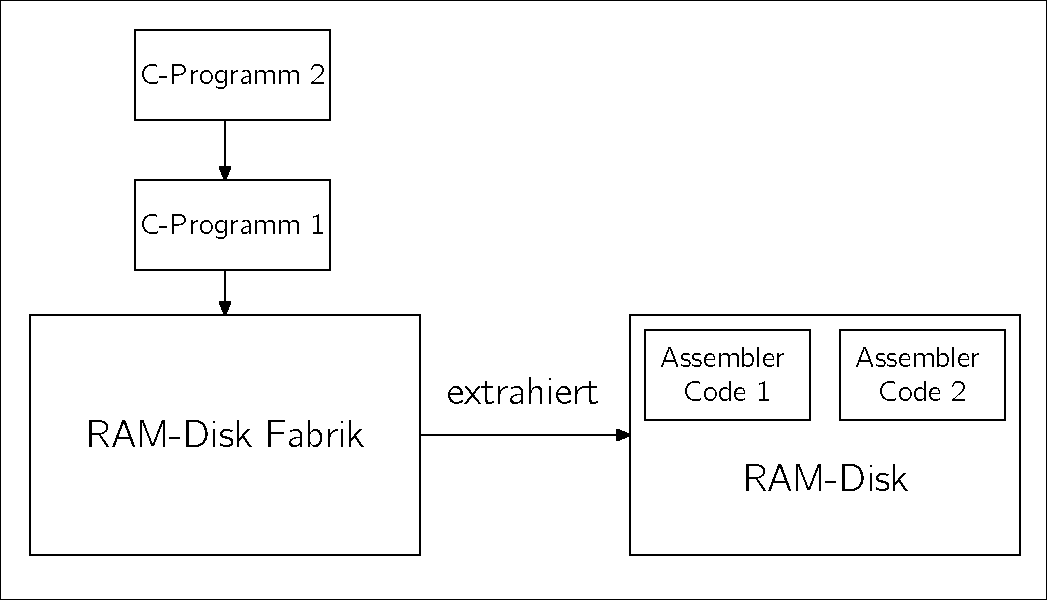
\includegraphics[scale=0.60]{common/draft-thread-ramdisk.pdf}	
	\caption{Erstellung der RAM-Disk}
	\label{draft:draft-thread-ramdisk}
\end{figure}
\noindent
Die Idee die in \mops verfolgt wurde bestand darin einfache C-Programme zu entwerfen und diese durch ein Programm zu schicken das den Assembler-Code dieser Programme extrahiert. In Abbildung \ref{draft:draft-thread-ramdisk} ist zu erkennen das zwei Programme durch die sogenannte RAM-Disk Fabrik wandern und diese extrahiert den Assembler-Code und verpackt ihn in die daf\"ur vorgesehene RAM-Disk. Der entstandene Assembler-Code kann dann von einem \mops -definierten Lader in den Speicher bef\"ordert werden.\\\\
Neben dem vorbereiten und Laden der Threads in den RAM ist es aber auch notwendig die Threads zu verwalten. Diese Aufgabe \"uebernimmt unter anderem der Kernel.
\section{Kernel}
Der Kernel ist der Teil von \mops der s\"amtliche Verwaltungsaufgaben \"ubernimmt die man sich vorstellen kann. Das geht von den Interrupts bis hin zur Verwaltung der Threads.
\begin{figure}[h!]
	\centering
	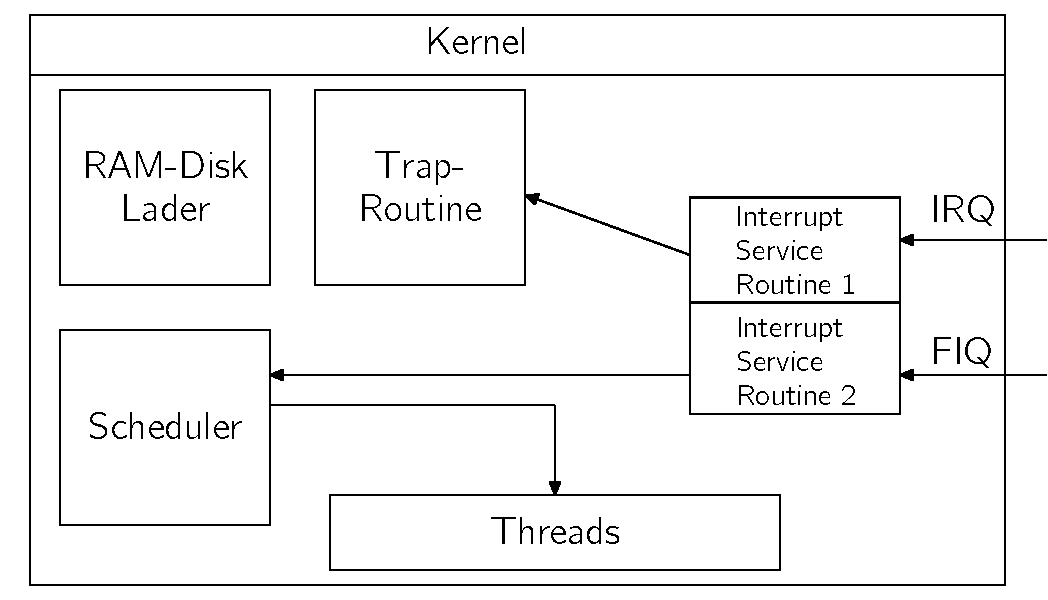
\includegraphics[scale=0.60]{common/draft-kernel.pdf}	
	\caption{Kernel - \"Uberblick}
	\label{draft:draft-kernel}
\end{figure}\newpage\noindent
Die Abbildung \ref{draft:draft-kernel} gibt nochmal eine detailierten Einblick in das Innenleben des Kernels. Zu sehen sind hier alle Komponenten die auf die Idee mit Einfluss hatten. Der RAM-Disk Lader, Interrupt-Service Routinen, der Scheduler und die Trap-Routinen. Diese Abbildung soll darstellen wie ein normaler Ablauf in dem Kernel aussehen kann. \\
Im ersten Schritt kommt ein Interrupt oder Fast-Interrupt-Request in das System, der Interrupt-Controller priorisiert diesen dann und stellt dem Kernel die passende Interrupt-Service Routine zur Verf\"ugung. Die jeweilige Routine kann dann z.B. entweder einen Trap-Routine Aufrufen oder aber, was wesentlich interessanter ist, den Scheduler. Dieser Scheduler geht dann an die Thread-Tabelle und greift sich einen neuen Thread der jetzt in den Prozessor geladen wird. Womit wir beim n\"achsten Punkt sind.\\ \\
Der Scheduler ist ein Manager f\"ur die Verwaltung der Prozessorzeiten und Priorisierung der Threads.
\begin{figure}[h!]
	\centering
	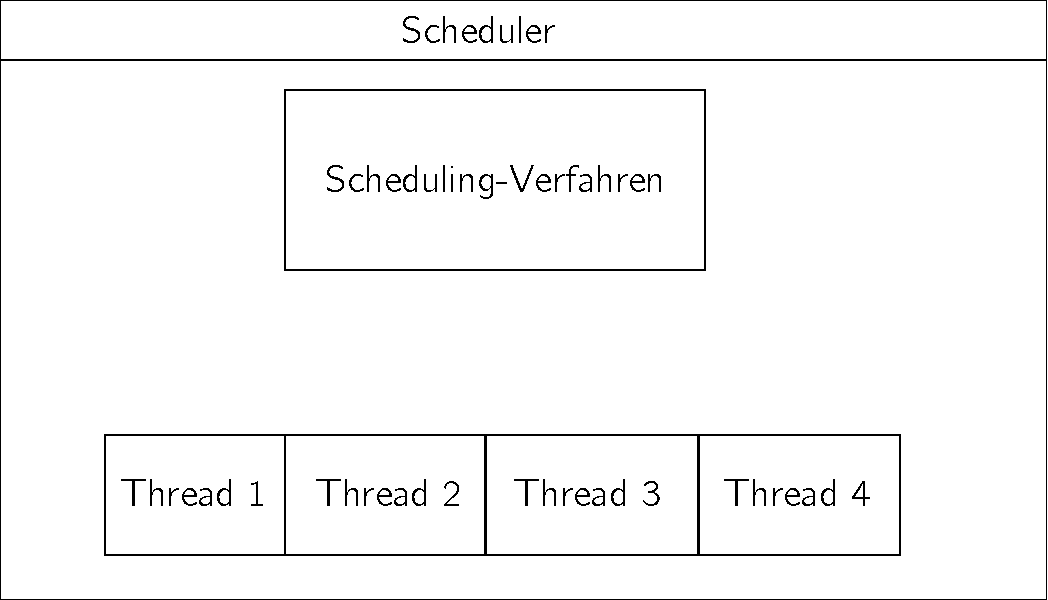
\includegraphics[scale=0.60]{common/draft-scheduler.pdf}	
	\caption{Scheduler}
	\label{draft:draft-scheduler}
\end{figure}\\
Er setzt sich aus zwei wichtigne Komponenten zusammen. Dem Scheduling-Verfahren, welches frei gew\"ahlt werden kann und einer Tabelle von Threads. Aus dieser Tabelle w\"ahlt der Scheduler, je nach Scheduling-Verfahren, einen Thread aus und \"ubergibt ihm die Kontrolle. Es gibt viele Scheduling-Verfahren, aber hier wurde sich jedoch einer Idee bedient die in der fr\"uhzeitigen Entwicklung von Schedulern weit verbreitet war. 
\newpage\noindent
Das Verfahren nennt sich \textbf{Round-Robin-Verfahren}. Die folgende Grafik soll das Verfahren beschreiben.
\begin{figure}[h!]
	\centering
	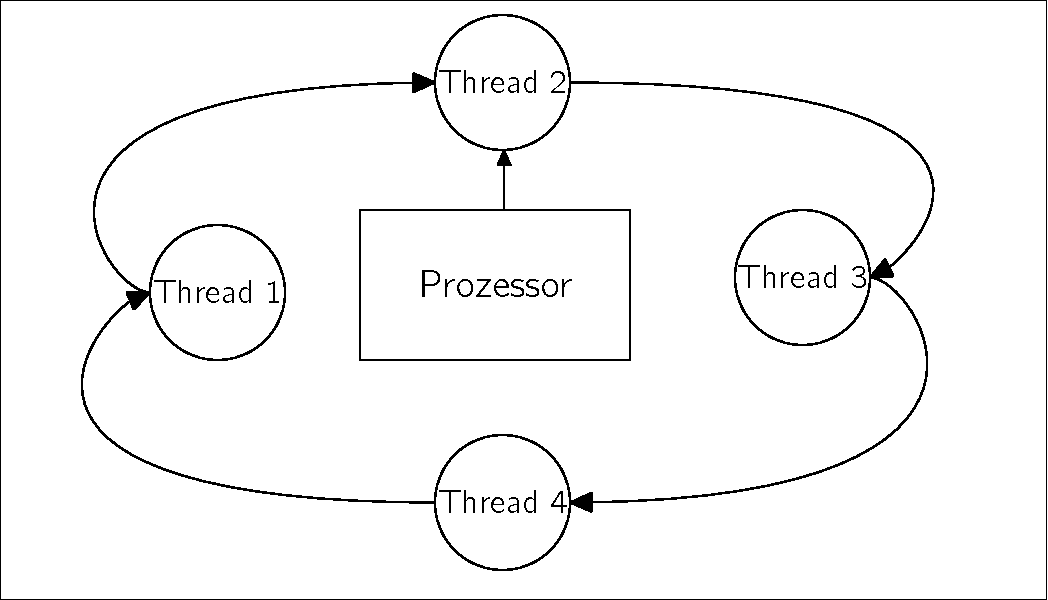
\includegraphics[scale=0.60]{common/draft-roundrobin.pdf}	
	\caption{Round-Robin Verfahren - Schematisch}
	\label{draft:draft-roundrobin}
\end{figure}\\
Beim Round-Robin Verfahren wird der Scheduler so entwurfen das er jedem Thread eine fixe Zeitspanne an Prozessorzeit zusichert und die Kontrolle dann an den jeweiligen Thread \"ubergibt. Nach Ablauf der Zeit wird dann der n\"achsten Thread in der Tabelle aufgerufen. Diese Verfahren wurde f\"ur \mops deshalb gew\"ahlt weil in Handheld Ger\"aten keine Sonderpriorisierungen stattfinden m\"ussen und die Umsetzung in den Zeitrahmen passte.